\section{Prefazione}\label{prefazione}

\subsection{Abstract}\label{abstract}

This research aims to investigate over a coherent way to extract
geographical information by the Decameron's novels of Boccaccio using
modern tools.

\subsection{Keywords}\label{keywords}

computational linguistics; reproducible research;

\subsection{Aknowledgments}\label{aknowledgments}

Progetto parzialmente finanziato grazie al grant XXX dell'Università
YYY.

\section{Introduzione}\label{introduzione}

\section{Brevi note sullo stato dell'arte nella geografia del
Decameron}\label{brevi-note-sullo-stato-dellarte-nella-geografia-del-decameron}

Una delle caratteristiche principali del \emph{Decameron} di Giovanni
Boccaccio è senza dubbio l'enorme varietà geografica presente
nell'opera: l'autore infatti cita innumerevoli paesi, città, piccoli
borghi o addirittura luoghi fantastici, che all'interno delle cento
novelle rappresentano ambientazioni o anche soltanto rapidi accenni. Un
incredibile paesaggio si delinea dunque tra le pagine di quest'opera,
che stimola continuamente l'interesse del lettore a spostarsi tra
Firenze, Napoli, Bologna, a tuffarsi nel Mediterraneo, a risalire
l'Europa sino in Irlanda, e a immaginare un esotico oriente nel cinese
Catai (X 4) \footnote{Ove non diversamente indicato, l'edizione
  decameroniana di riferimento è stata, per tutte le citazioni di questo
  articolo, la seguente \autocite{boccaccio2013decameron}. La citazione
  in corpo al testo segue il modello giornata (in numero romano),
  novella e, dove necessario, paragrafo} «una geografia così immensa e
irrequieta, così gioiosa di vagabondare, da novella a novella e
all'interno di una stessa novella \autocite{getto1972vita}. In merito
alla geografia, la storia della critica decameroniana si è espressa in
maniera saltuaria e difforme: il primo studio realmente focalizzato su
questo argomento è arrivato soltanto nel 2011: si tratta dell'importante
miscellanea di studi dal titolo \emph{Boccaccio geografo}, a cura di
Roberta Morosini \autocite{morosini2010boccaccio}. Proprio dai
contributi a questo testo si traggono numerose notizie riguardo al mondo
geografico del Certaldese \footnote{Per un approfondimento più
  esauriente sulle suggestioni, le fonti letterarie, il materiale
  geografico circolante nel Trecento e le opere coeve di Boccaccio,
  rimandiamo anche a \autocite{bolpagni2016} e in particolare alle
  pp.~16-36}.

In questa sede appare doveroso soltanto ricordare brevemente che
l'interesse geografico di Boccaccio nasce da stimoli diversi, quasi
tutti provocatigli dal contatto con la corte di Re Roberto d'Angiò a
Napoli. Qui il certaldese trascorse gli anni della sua formazione e
giovinezza: vi giunse infatti quattordicenne nel 1327, e tornò a
Firenze, a malincuore, solo nel 1341
\autocite[pp.~16-40]{branca1977giovanni}. Oltre alla frequentazione
della residenza reale, fonte di stimoli intellettuali e letterari
fondamentali per la formazione del poeta, durante il suo soggiorno
napoletano, Boccaccio ebbe modo di impratichirsi anche nell'arte del
commercio, lavorando a fianco del padre, agente dell'importante
compagnia commerciale fiorentina dei Bardi: il giovane si occupava di
lettere di credito, di cambio di monete, e di cassa. Spesso, inoltre, si
spostava dalla sua postazione per compiere varie commissioni dalla zona
portuale: proprio dall'approfondita conoscenza di Boccaccio di quei
luoghi nasce la perfetta ricostruzione ambientale della novella II 5,
ambientata nella Rua Catalana di Napoli, insieme con i suoi personaggi
più caratteristici, che ritroveremo poi nelle salaci rappresentazioni
dell'adescatrice palermitana madonna Iancofiore nella VIII 10, o di
Fiordaliso, finta sorella di Andreuccio, nella succitata novella
napoletana. È altamente probabile che la frequentazione quotidiana con
mercanti e gente proveniente dai più diversi paesi d'Occidente e
d'Oriente, abbia suscitato sin dall'inizio in Boccaccio una sensibilità
geografica che, pur basandosi, nella maggior parte dei casi, su racconti
orali di uomini d'affari, ha influito non poco sull'ambientazione
variegata dei luoghi decameroniani. Si è fatto spesso riferimento, in
sede critica, al cosidetto realismo delle novelle boccacciane, in cui
anche il misterioso Oriente diventa uno \emph{spazio sociale}
attendibile, nell'accezione proposta da Lefebvre, secondo il quale lo
spazio sociale è

\begin{quote}
l'incontro, l'unione, la simultaneità {[}\ldots{}{]} tutto ciò che è
prodotto dalla natura e dalla società {[}\ldots{}{]} esseri viventi,
cose, oggetti, opere, segni e simboli

\autocite[p.116]{lefebvre1978}
\end{quote}

Si può affrontare dunque uno spazio di viaggio avventuroso nel
Mediterraneo come seguendo un portolano mercantile, o un'ambientazione
veneziana come luogo in cui convogliano i peggiori sentimenti umani
\footnote{Proprio la II giornata, così peculiare e polare nelle sue
  peregrinazione attraverso il \emph{Mare Nostrum} sarà la protagonista
  di questo studio. Un'analisi narratologica basata sui metodi di
  ricognizione geografici automatici proposti nel prossimo capitolo
  verrà svolta in conclusione}.

Sovente in letteratura specializzata si accenna a un vago ``realismo''
decameroniano, termine ancora tutto da circoscrivere e ponderare. Posto
che, in questa sede, interessa soprattutto il realismo geografico, è
altresì innegabile che esso non possa essere disgiunto, almeno a livello
di descrizione e ambientazione, da quello storico o temporale: già negli
anni Sessanta la critica ha cominciato a sottolineare l'empirismo del
punto di vista di Boccaccio, che si preoccupa sempre, o quasi, di dare
ai suoi racconti il colore di fatti realmente accaduti, dove gli
ambienti sono sempre descritti meticolosamente, le situazioni sempre
giustificate e le famiglie spesso davvero esistite \footnote{Per uno
  studio fondamentale dell'empirismo ideologico e del realismo artistico
  di Boccaccio, cfr. \autocite[pp.~6-22]{1966decameron}. È una narrativa
  che spalanca le porte del realismo all'Occidente e che «tocca le
  radici dell'esperienza» \autocite[p.~229]{battaglia1993}}. Non essendo
comunque questa la sede per un \emph{excursus} sul realismo in
Boccaccio, ci limitiamo a segnalare come l'obiettivo di Boccaccio non è
documentaristico come potrebbe essere quello di un cronachista, ma
letterario, e dunque la definizione a nostro parere più congrua è quella
di Luigi Surdich, per il quale realismo realismo è

\begin{quote}
nominare con puntualità i personaggi delle singole narrazioni
{[}\ldots{}{]} circostanziando nel maggior numero possibile di casi
tempo storico, localizzazione, ambiente, e realismo è anche la motivata
reticenza di cui si fa carico Filomena

\autocite[p.~96]{surdich2008boccaccio}.
\end{quote}

Surdich ha osservato, a proposito della seguente introduzione
programmatica alla terza novella della terza giornata, che questo
scrupolo di Filomena, apparentemente classificabile come «protesta
frequente» \autocite[p.~347]{brancadecameron} o tutt'al più ascrivibile
alla tradizione, in realtà andrebbe ricondotto proprio al realismo
boccacciano, per il quale la censura sul nome dei protagonisti rivela il
timore di un riconoscimento scomodo e imbarazzante da parte della
brigata, il che sottolinea un'estrema volontà di rappresentazione del
mondo contemporaneo da parte dell'autore:

\begin{quote}
Nella nostra città, più d'inganni piena che d'amore o di fede, non sono
ancora molti anni passati, fu una gentil donna di bellezze ornata e di
costumi, d'altezza d'animo e di sottili avvedimenti quanto alcuna altra
dalla natura dotata, il cui nome, né ancora alcuno altro che alla
presente novella appartenga come che io gli sappia, non intendo di
palesare, per ciò che ancora vivon di quegli che per questo si
caricherebber di sdegno, dove di ciò sarebbe con risa da trapassare (III
3,5).
\end{quote}

Tuttavia, sarebbe forse ingenuo considerare questa reticenza di Filomena
come realmente ispirata da fatti di cronaca: si tratta infatti di un
realismo che fa ricorso «alla solidificazione dei pregiudizi e alla
memoria culturale» \autocite[p.~97]{surdich2008boccaccio}. Bastino come
esempi, per ora, la prassi fiorentina antica delle brigate, ricordata
nella novella VI 9 di Guido Cavalacanti, la nomea delle brutte donne di
Pisa (II 10) o ancora i percorsi mediterranei dei mercanti italiani
ricalcati pedissequamente dalle rotte di Alatiel nella II 7: tutte
queste occorrenze, insieme a molte altre, sono indicative di un realismo
piuttosto teso all'edificazione di una storia credibile, anche alla luce
egli obbiettivi narrativi che Boccaccio si pone. Decisamente esplicativa
è, in questo senso, l'introduzione della quinta novella della nona
giornata da parte di Fiammetta, che afferma:

\begin{quote}
Se io dalla verità del fatto mi fossi scostare voluta o volessi, avrei
ben saputo e saprei sotto altri nomi comporla e raccontarla; ma per ciò
che il partirsi dalla verità delle cose state nel novellare è gran
diminuire di diletto negl'intendenti, in propria forma, dalla ragion di
sopra detta, la vi dirò (IX 5,5).
\end{quote}

Il \emph{diletto degli intendenti} dunque, si profila come fine
principale della narrazione del Boccaccio, che non si preoccupa, come
invece avviene in opere erudite come ad esempio nel \emph{De montibus}
\autocite{demontibus}, di rispettare ad ogni costo l'aderenza alle fonti
o alla realtà oggettiva e sperimentata (nel caso del trattato suddetto,
più le prime che la seconda), ma piuttosto segue regole narrative
proprie diletto (e della novella).

La curiosità dell'autore nei confronti dell'alterità, soprattutto
orientale, è stata stimolata anche da diversi accadimenti storici a
cavallo dei secoli XIII e XIV: tra essi, possiamo ricordare l'incontro
tra la civiltà cristiana e quella araba in Spagna e in Sicilia, le
Crociate e i pellegrinaggi in Terra Santa, l'invasione e instaurazione
dell'impero dei Mongoli \autocite[p.~20]{morosini2010boccaccio}. La
bibliografia in merito è realmente vasta: tuttavia, se dovessimo
segnalare i punti fermi della critica ai quali ci siamo affidati nel
corso di tutto il lavoro, essi senza dubbio corrisponderebbero da una
parte all'introduzione di Vittore Branca all'edizione Einaudi del
\emph{Decameron}, e dall'altra al capitolo \emph{Le coordinate
spazio-temporali del racconto} inserito da Alberto Asor Rosa nel suo
saggio per la collana \emph{Letteratura Italiana} pubblicata da Einaudi
\autocite{asor1992}. Branca è stato il primo a sottolineare sia la
centralità di Firenze (e la corrispondente declinazione delle zone
geograficamente secondarie) che la caratterizzazione geolinguistica che
contraddistingue determinati personaggi, per esempio a Venezia o a
Siena. Asor Rosa, invece, ha fornito interessanti raggruppamenti
schematici delle novelle a seconda del luogo di ambientazione,
distinguendo questa in primaria e secondaria, e creando delle apposite
categorie per Firenze, il quadro italiano e il mondo extranazionale.
Inoltre, lo studioso in questione ha suggerito delle tabelle schematiche
anche per le funzioni di viaggi, che sarà nostro interesse aggiornare
con nuove definizioni. Un quadro geografico così vario come quello del
Decameron comprova non solo l'ampiezza e la varietà del mondo nel quale
il Boccaccio fa muovere e agire i personaggi delle sue cento novelle, ma
anche gli interessi vivissimi, l'apertura mentale, l'efficienza e la
vitalità che caratterizzano le loro azioni e i loro atteggiamenti.

\begin{quote}
Questo vuol dire, in conclusione, che i luoghi geografici non sono
meccaniche collocazioni dell'azione in un ambito qualsiasi determinato
spazialmente, ma rappresentano dimensioni e simboli dell'immaginario,
conformati in modo tale da cogliere ed esprimere le fantasie
dell'autore. Ognuno dei luoghi boccacciani produce un proprio adeguato
immaginario e orienta le soluzioni narrative conseguenti
\end{quote}

\begin{quote}
\autocite[p.~548]{asor1992}.
\end{quote}

Ci sarebbe dunque, concretissimo, un rapporto tra le ambientazioni delle
storie narrate dalla brigata e i suoi personaggi, come se i luoghi
geografici influenzassero le azioni dei protagonisti? La risposta è
duplice. Infatti, come si è constatato in un recente contributo a firma
di chi scrive \autocite{bolpagni2016}, è possibile creare un
parallelismo strutturale tra l'astuzia dei personaggi e la città di
Firenze, mentre dall'altra parte alcuni pregiudizi e inimicizie
storico-politiche fanno sì che Venezia, Siena e altre realtà siano
popolate da gente piuttosto sciocca. Questa visione geografica
amplissima non contrasta affatto con la scelta di un centro costituito
dalla Toscana e, in particolare, dalla succitata Firenze, che troneggia
come ambientazione principale non solo in numerose novelle dell'opera,
ma anche nella cornice stessa, proponendosi come l'alfa e l'omega
geografico del Decameron, in un processo di \emph{Ringkomposition} che
spesso investe anche la maggior parte dei viaggi interni alle novelle
\footnote{Per un contributo dettagliato e aggiornato della distribuzione
  dei luoghi nelle varie novelle del \emph{Decameron} vd.
  \autocite[p.~93]{cavallini2002}. Tuttavia, non dimentichiamo che la
  relatività della visione è d'obbligo: cfr. il contributo succitato di
  A. Asor Rosa, che sottolinea invece l'importanza delle settanta
  novelle extratoscane della raccolta da una parte, e l'esclusione
  pressoché totale di Firenze dagli esempi di virtù della decima
  giornata}.

Proprio i viaggi, soprattutto nella loro declinazione mediterranea e,
per quel che può significare il concetto di Italia nella geografia
medievale \footnote{È saggio tenere presente che, almeno fino al XV
  secolo, la geografia medievale non si caratterizza, come quella
  moderna, per una dimensione temporale di lunga durata: essa è
  immutabile, e provvidenziale, e si basa piuttosto su una continua
  allegoria per la quale lo spazio fisico rimanda a quello della fede,
  che lo contiene, limita e conferma. Questo significa che viaggiatori
  come Guglielmo di Rubruck, Odorico da Pordnenone e lo stesso Marco
  Polo si preoccupavano piuttosto di ritrovare negli spazi che
  scoprivano luoghi o popoli citati dal Pentateuco o dai libri storici
  della Bibbia o dai profeti. Dall'altra parte però, l'interesse verso
  il mondo orientale era stato preparato anche da quella tendenza
  culturale comunemente chiamata \emph{translatio studii}. Si tratta in
  sostanza dello slittamento storico dall'est all'ovest dei centri di
  potere e di sapere: tra le opere tradotte in latino a partire dal XII
  secolo, ricordiamo il Corano a cura di Pietro il Venerabile, la
  traduzione in francese del \emph{Roman de Mahomet} negli anni
  1250-1260 da parte del chierico Alexandre du Pont e, nello stesso
  periodo, l'anonima versione latina dell'\emph{Historia orientalis} del
  vescovo di Acri Giacomo di Vitry}, costituiscono un \emph{fil rouge}
che attraversa la raccolta boccacciana e che si pone ormai da tempo come
oggetto privilegiato di attenzione critica. Perché dunque non prendere
le mosse dalla proposta, avanzata da Giulio Ferroni, di una geocritica
della letteratura, cioè di una disciplina che configuri

\begin{quote}
una coscienza dello spazio, modi mentali di riconoscere e misurare la
spazialità e la consistenza stessa dei luoghi, proiezioni e combinazioni
che alterano la percezione dello spazio esterno {[}\ldots{}{]}
\emph{laddove} lo spazio letterario può essere concepito anche come
{[}\ldots{}{]} una misura ``altra dello spazio''

\autocite[p.~90]{ferroni2012}
\end{quote}

Ferroni, poche righe dopo, sottolinea anche la mancanza di uno studio
che illustri la diversa configurazione dei luoghi nelle grandi opere
della letteratura italiana. Per quanto improba appaia a livello globale
l'appello lanciato qui sopra, pensiamo che siano proprio le novelle di
viaggio a poter costituire un punto di partenza per un'analisi
narratologica degli spostamenti geografici diegetici a partire da dati
reali. Come isolare dunque, sfuggendo a catalogazioni arbitrarie, le
storie effettivamente impattanti dal punto di vista del viaggio e, non
meno impellente, come selezionarle in maniera processabile
computazionalmente? La visualizzazione grafica dei luoghi decameroniani
e degli spostamenti diegetici all'interno delle storie è una delle sfide
che ci poniamo a monte di questo studio. L'obiettivo, dunque, sarà
quello di creare delle mappe coropletiche (cioè mappe tematiche in cui
le aree sono diversamente colorate o graficamente rappresentate in modo
da evidenziare i risultati di calcoli statistici effettuate su di esse),
che illustrino i percorsi mediterranei (e non) dei protagonisti delle
novelle. Il tutto attraverso strumenti automatici di processazione dei
dati. Questa scelta di rappresentare graficamente sia i calcoli sia le
rotte decameroniane risponde in primo luogo ad un'esigenza di chiarezza
e comprensibilità da offrire al lettore anche non specializzato in
ottica divulgativa, dall'altra vuole avvicinare la geografia letteraria
e qualsiasi considerazione successiva intorno al valore morale dello
spazio alle nuove discipline delle \emph{digital humanities}, che
prevedono la digitalizzazione di viaggi letterari su supporti
informatici e la loro interrogabilità. La scelta di un tale approccio
computazionale, che verrà sviscerato nel seguente capitolo, vuole porsi
anche come un tentativo di interdisciplinarietà che vede nella
riproducibilità e applicabilità dei modelli il suo punto di forza. Per
quanto riguarda la scelta delle novelle,la proposta di classificazione
di Asor Rosa è a questo proposito convincente, isolando egli un gruppo
di storie, prevalentemente inserite nella seconda giornata, in cui «il
viaggio ha un rapporto assolutamente intrinseco con la narrazione»
\autocite[p.~549]{asor1992}. Secondo questa categoria, le novelle elette
sarebbero: II 3 (i tre fratelli scialacquatori e il nipote Alessandro
che sposerà la figlia del re d'Inghilterra); II 4 (Landolfo Rufolo); II
6 (madama Beritola); II 7 (Alatiel); II 8 (Il Conte d'Anguersa); II 9
(Zinevra e Bernabò); III 9 (Giletta di Nerbona e Beltramo), IV 3 (Tre
giovani amano tre sorelle); V 1 (Cimone); V 2 (Gostanza e Martuccio); V
3 (Pietro Boccamazza e l'Agnolella); V 6 (Gian di Procida) e X 9 (Il
Saladino e messer Torello). Tutti i protagonisti di queste storie sono,
per i più svariati eventi della sorte, impegnati in un viaggio: ma solo
alcuni di loro lo sperimentano come «barriera potenziale» \footnote{L'autore
  di questa definizione è Dmitrij S. Lichačëv, all'interno di
  \autocite[pp.~26-39]{lotman1973}, come «stupefacente metafora del
  vissuto» \autocite[p.~550]{asor1992}.}. Tuttavia, non tutte le novelle
succitate si svolgono in ruoli ``altri''. Rispettivamente, la storia di
Beritola, quella di Pietro Boccamazza e quella di Gian di Procida
rimangono all'interno dei confini nazionali, pur proponendo, tranne che
nella V 3, spostamenti mediterranei. Tuttavia, se le peripezie di
madonna Beritola saranno funzionali sia alla rappresentazione grafica
degli spostamenti decameroniani, ormai uno degli obiettivi dichiarati di
questo lavoro, sia per trarre conclusioni narratologiche (come si
vedrà), ci sentiamo di escludere dal computo le novelle V 3 e V 6 le
quali, pur basandosi su un viaggio, offrono itinerari troppo
circoscritti per poter risultare esemplari. Ecco dunque che in rilievo,
quasi spontaneamente, fa capolino la seconda giornata, nella quale, come
già rilevato, il rapporto con il viaggio è essenzialmente intrinseco
\autocite{zatti2004}. Forti dei motivi di rappresentazione e
riproducibilità suddetti, sarà dunque questa la porzione decameroniana
oggetto delle analisi che seguono.

\section{L'approccio digitale: orizzonti e
metodi}\label{lapproccio-digitale-orizzonti-e-metodi}

\begin{itemize}
\tightlist
\item
  Approccio quantitativo/ qualitativo.
\item
  ASTRAZIONE: trasformare un testo in lista di vettori
\item
  Come si fa una sottrazione tra coordinate?
\item
  Metodo di lavoro: l'approccio computazionale. Quali sono i vantaggi e
  i metodi.
\end{itemize}

\subsection{Testi, corpora, dati}\label{testi-corpora-dati}

\autocite{owens2011}

bla

\autocite{moretti2005}

\subsection{Gli strumenti usati}\label{gli-strumenti-usati}

L'indagine preliminare ha previsto l'estrazione di una porzione iniziale
del testo dell'opera, usata come \emph{campione d'indagine} per testare
la validità e la correttezza degli strumenti informatici a disposizione
in rapporto con i risultati attesi e lo stile linguistico del testo in
esame\footnote{Risulta necessario sottolineare, e lo faremo in maniera
  più esplicita nel corso dell'articolo, quanto l'uso di software e
  librerie designate per l'analisi del linguaggio odierno possa creare
  delle problematicità evidenti se riferite a testi antichi.}. Tale
campione estratto dal proemio alla prima giornata --di per sé non
rappresentativo-- consta di 267 parole nell'edizione di riferimento ed i
suoi confini sono rappresentati dalle espressioni: «Umana cosa», «guisa
che sol di sé» \footnote{Le analisi sono state effettuate su laptop
  equipaggiato con processore Intel(R) Core(TM) I5 M480 2.67GHz 64bit,
  8GB RAM DDR3, OS: Linux Lubuntu 17.10, HD 1TB 5400rpm; compilatori per
  diversi linguaggi, tra cui Python e R.}.

La prima operazione è stata quella di rintracciare gli strumenti
informatici che meglio potessero supportare le operazioni necessarie
all'estrazione delle informazioni ai fini dell'analisi in oggetto. Le
alternative principali che abbiamo valutato sono rappresentate da 4 tool
di trattamento automatico del linguaggio (\emph{Natural Language
Processing} (NLP)), che andremo a discutere di seguito:

\begin{itemize}
\item
  UDPipe \autocite{udpipe2017}\\
  Elaborato presso l'Università di Praga, UDPipe è un tool versatile che
  permette l'annotazione, il tagging, la lemmatizzazione e il parsing
  delle dipendenze sintattiche del documento, attraverso il caricamento
  di appositi dataset elaborati nella lingua-modello. Rilasciato con
  licenza aperta Mozilla Public License 2.0, accoglie nativamente la
  possibilità di lettura ed esportazione di file in formato standard
  CoNLL-U; è disponibile per Linux/ Windows/ OS X, come libreria per
  C++, Python, Perl, Java, C\#, R e come servizio web. Nella presente
  analisi è stato utilizzato come libreria per ambiente R.
\item
  ItaliaNLP\\
  Interfaccia Web
\item
  TreeTagger \autocite{schmid1994b}\\
  TreeTagger è un tagger di tipo probabilistico, disponibile per
  Windows/ Linux/ OS X e con contenitori per differenti ambienti --R,
  Python, Java-- e come applicazione standalone per Windows. La pipeline
  mostra un parser ed una serie di \emph{modelli} di lingua da caricare
  nel motore per performare le analisi. Lo abbiamo utilizzato grazie
  all'agevole interfaccia web messa a disposizione dall'Università degli
  Studi di Perugia.
\item
  PATTERN \autocite{pattern2012}\\
  Specificatamente pensato per il \emph{mining} di informazioni dal Web,
  prevede uno scraper di informazioni dalla DOM delle pagine HTML per
  l'estrazione del testo. Permette di avviare indagini di sentiment
  analysis, oltre alle operazioni più classiche di lemmatizzazione e
  POS-tagging; è disponibile per ambiente Python.
\end{itemize}

Si è proceduto dunque con l'operazione di lemmatizzazione automatica,
comparando i vari tool. In questo modo le singole parole del testo, o
\emph{tokens}, vengono ricondotte dalla loro forma al lemma
corrispondente. La tabella seguente mostra il tasso di uguaglianza tra i
tool in termini assoluti sulle 267 forme:

\begin{longtable}[]{@{}llll@{}}
\toprule
& ItaliaNLP & TT(UniPG) & PATTERN\tabularnewline
UDPIPE & 240 & 203 & 223\tabularnewline
ItaliaNLP & & 219 & 231\tabularnewline
TT(UniPG) & & & 198\tabularnewline
\bottomrule
\end{longtable}

Successivamente si è optata la scelta della valutazione manuale della
correttezza dei tool, al fine di determinare quale tra gli strumenti in
esame potesse meglio adattarsi all'analisi del documento in oggetto. La
valutazione manuale, riportata di seguito, è stata elaborata sotto forma
di percentuale rispetto al totale del campione, e vede UDPipe come
quello che più fedelmente si è avvicinato ad un livello compatibile con
i risultati attesi, sebbene la difficoltà di un testo antico.

\begin{figure}
\centering
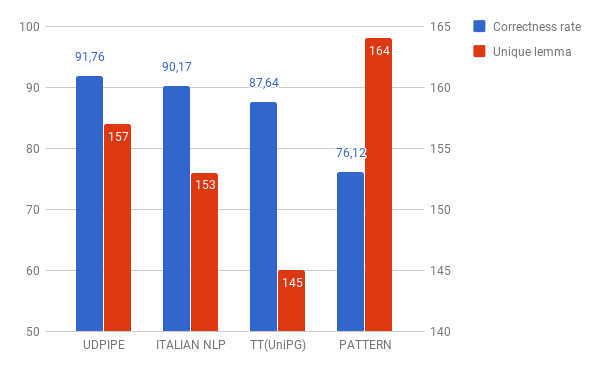
\includegraphics[width=0.70000\textwidth]{../charts/correctnessLib-Lemma.png}
\caption{Grafico di comparazione della correttezza dei lemmi
riconosciuti automaticamente}
\end{figure}

\subsection{La pipeline di lavoro}\label{la-pipeline-di-lavoro}

\section{Narratologia}\label{narratologia}

\begin{itemize}
\tightlist
\item
  Lo spostamento dei personaggi e/o della narrazione all'interno di una
  novella prevede direzioni più frequenti di altre? (es. est-ovest,
  nord-sud)
\item
  Possiamo identificare delle tendenze migratorie nella seconda
  giornata?
\item
  la seconda giornata è realmente una sequela di avventure e di
  migrazioni o potremmo piuttosto definirla un ben orchestrato gruppo di
  ritorni a casa?
\item
  I personaggi che si allontanano di più dal luogo di partenza
  acquisiscono capacità come in un tradizionale \emph{Bildungsroman} ? O
  piuttosto perdono le loro certezze a contatto con l'alterità?
\item
  Limitatamente alla seconda giornata, possiamo stabilire se Boccaccio
  propone dei viaggi di pura avventura e \emph{divertissement} o se sono
  applicabili delle prospettive metaforiche?
\end{itemize}

\section{Conclusioni}\label{conclusioni}

\section{Risorse}\label{risorse}

\subsection{Maps}\label{maps}

\begin{figure}
\centering
\includegraphics{https://github.com/olablit2/geoBoccaccio/raw/master/data/out/maps/0201.png}
\caption{figure}
\end{figure}

\begin{figure}
\centering
\includegraphics{https://github.com/olablit2/geoBoccaccio/raw/master/data/out/maps/0202.png}
\caption{figure}
\end{figure}

\begin{figure}
\centering
\includegraphics{https://github.com/olablit2/geoBoccaccio/raw/master/data/out/maps/0203.png}
\caption{figure}
\end{figure}

\begin{figure}
\centering
\includegraphics{https://github.com/olablit2/geoBoccaccio/raw/master/data/out/maps/0204.png}
\caption{figure}
\end{figure}

\begin{figure}
\centering
\includegraphics{https://github.com/olablit2/geoBoccaccio/raw/master/data/out/maps/0205.png}
\caption{figure}
\end{figure}

\begin{figure}
\centering
\includegraphics{https://github.com/olablit2/geoBoccaccio/raw/master/data/out/maps/0206.png}
\caption{figure}
\end{figure}

\begin{figure}
\centering
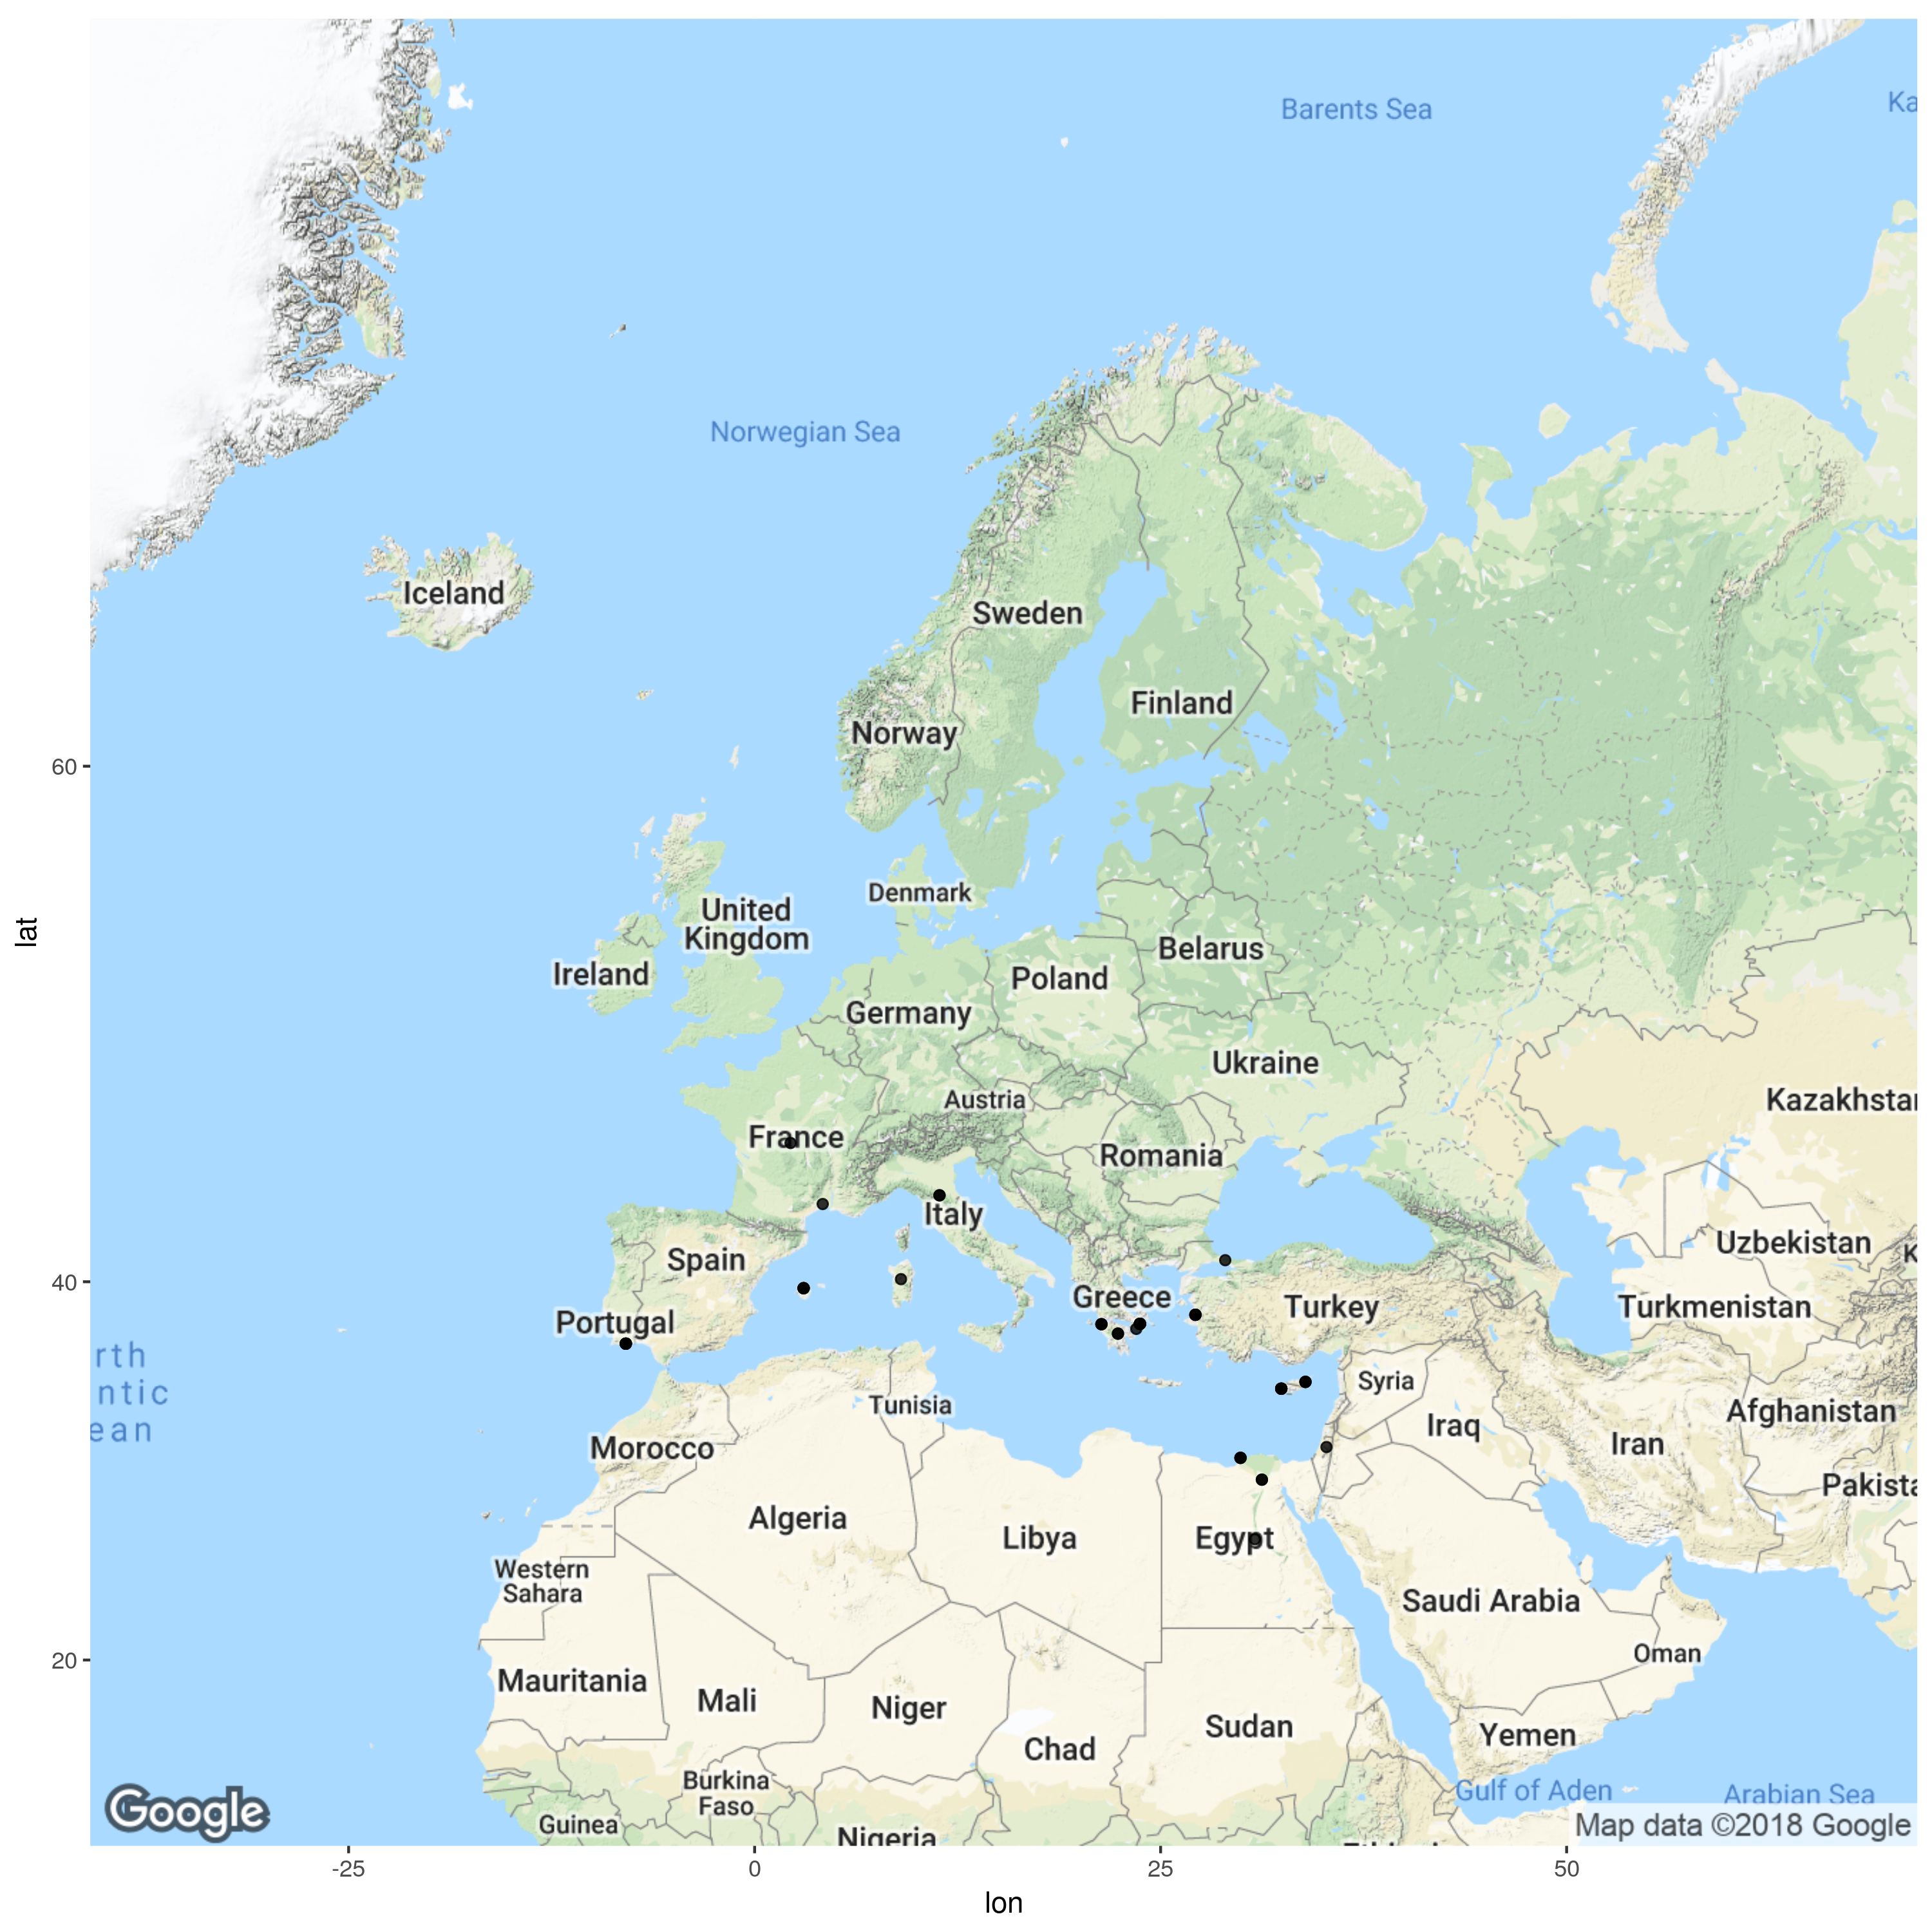
\includegraphics{https://github.com/olablit2/geoBoccaccio/raw/master/data/out/maps/0207.png}
\caption{figure}
\end{figure}

\begin{figure}
\centering
\includegraphics{https://github.com/olablit2/geoBoccaccio/raw/master/data/out/maps/0208.png}
\caption{figure}
\end{figure}

\begin{figure}
\centering
\includegraphics{https://github.com/olablit2/geoBoccaccio/raw/master/data/out/maps/0209.png}
\caption{figure}
\end{figure}

\begin{figure}
\centering
\includegraphics{https://github.com/olablit2/geoBoccaccio/raw/master/data/out/maps/0210.png}
\caption{figure}
\end{figure}

\section{Temporaneo}\label{temporaneo}

\subsection{Roadmap}\label{roadmap}

\subsubsection{Objectives}\label{objectives}

This research aims to investigate over a coherent way to extract
geographical information in the narrative storytelling of Decameron 2nd
day novelle by the perspective of the narration (extra-diegetic /
fabula).

\subsubsection{Pipeline}\label{pipeline}

Preliminary steps * {[}DONE{]} Collect the corpus in a textual form
(e.g.~liberliber) * {[}DONE{]} Clean the corpus * {[}DONE{]} Divide the
corpus into partials (e.g.~0207.txt, 0203.txt \textbar{} namefile:
NNnn.txt where NN=02) * Tools testing * {[}DONE{]} POS and Lemmatization
correctness rate =\textgreater{} UDPIPE wins

\subsubsection{Geographic information}\label{geographic-information}

\begin{itemize}
\tightlist
\item
  {[}DONE{]} Use UDPIPE with the 10 subcorpora. Write the relative
  CONLL-U files of each partials
\item
  {[}DONE{]} Extract all the PROPN \textbar{} SP tokens for each
  partials
\end{itemize}

Using R

\begin{verbatim}
    infile <- read.csv(CONNLU)
    df <- infile[infile[,4] == "PROPN", ]
    write.csv(df, outfile)
\end{verbatim}

(Using G Spreadsheet)

\begin{verbatim}
    =query({IMPORTRANGE("https://docs.google.com/spreadsheets/d/1Qh7mGzfW2ow8RzOniqO_-60JST6pbT71dfzaz_GtV0k";"prova!A1:J15000")}; "SELECT * WHERE Col5 CONTAINS'SP'";0)
\end{verbatim}

\subsection{Merge the various csv}\label{merge-the-various-csv}

All the csv in the folder are merged into a total one. Alphabetically
ordered

\begin{verbatim}
mlr --csv --rs lf --csv sort -f date,code *.csv > total/final.csv
\end{verbatim}

\begin{itemize}
\tightlist
\item
  The given spreadsheets yields for a list of items of PNs. Order the
  list alphabetically. Insert a manual column where the token is
  standardized and give the relevant coords:
\end{itemize}

\begin{longtable}[]{@{}llll@{}}
\toprule
Item & Std & Long & Lat\tabularnewline
\midrule
\endhead
Vinegia & Venezia & 45.4042008 & 12.1015609\tabularnewline
\bottomrule
\end{longtable}

\begin{itemize}
\tightlist
\item
  Don't delete PNs which are not strictly relevant to the actual
  recognition: they serve as tools for tracing out the correctness rate
  or other info.
\item
  Give parallel spreadsheets for each partials which yields a structured
  array of PNs in texts. When merged with the previous one, it will
  results for 3 columns of each term: the ones which have coords field
  are the locations
\item
  Add a manual field to the spreadsheet which explicits the actors of
  that location
\end{itemize}

\begin{longtable}[]{@{}lllll@{}}
\toprule
Item & Std & Long & Lat & Actor\tabularnewline
\midrule
\endhead
Vinegia & Venezia & 45.4042008 & 12.1015609 & Buffalmacco\tabularnewline
\bottomrule
\end{longtable}

\begin{itemize}
\tightlist
\item
  Plot locations in map
\item
  Use the frequency list for the whole day
\end{itemize}

\subsection{Questions}\label{questions}

\begin{itemize}
\tightlist
\item
  Lo spostamento dei personaggi e/o della narrazione all'interno di una
  novella prevede direzioni più frequenti di altre? (es. est-ovest,
  nord-sud)
\item
  Quali le conseguenze narratologiche e morali di uno spostamento?
\item
  Possiamo identificare delle tendenze migratorie nella seconda
  giornata?
\end{itemize}

\subsection{Note}\label{note}

\begin{itemize}
\item
  Standardizzazione 17.7:
\item
  I ``Castel'' è da contestualizzare
\item
  II ``Grignano'' non lo so
\item
  III ``Ruga'' e ``Catalana'' valgono come un luogo (Napoli
\item
  IV ``Cresci'' e ``Valcava'' calgono come un luogo (Borgo S. Lorenzo)
\end{itemize}

prova marco

\href{https://github.com/olablit2/geoBoccaccio/edit/master/docs/2018-article/index.md}{EDIT
FILE}

\section{Nuove prospettive per lo studio della toponomastica nel
Decameron}\label{nuove-prospettive-per-lo-studio-della-toponomastica-nel-decameron}

\textbf{Marcello Bolpagni}, \textbf{Marco Petolicchio}

\begin{itemize}
\tightlist
\item
  Dept. of General Linguistics, Palacky University Olomouc;
  marcello.bolpagni@gmail.com
\item
  Dept. of Romance Languages, Palacky University Olomouc;
  marco.petolicchio01@upol.cz; ORCID: 0000-0001-7017-7862
\end{itemize}

\subsection{Struttura}\label{struttura}

\begin{itemize}
\tightlist
\item
  \href{https://olablit2.github.io/geoBoccaccio/2018-article/05-preface}{Prefazione}
\item
  \href{https://olablit2.github.io/geoBoccaccio/2018-article/10-introduction}{Introduzione}
\item
  \href{https://olablit2.github.io/geoBoccaccio/2018-article/20-chapter1}{Ch.1}
\item
  \href{https://olablit2.github.io/geoBoccaccio/2018-article/30-chapter2}{Ch.2}
\item
  \href{https://olablit2.github.io/geoBoccaccio/2018-article/40-chapter3}{Ch.3}
\item
  \href{https://olablit2.github.io/geoBoccaccio/2018-article/50-chapter4}{Ch.4}
\item
  \href{https://olablit2.github.io/geoBoccaccio/2018-article/90-conclusion}{Conclusioni}
\item
  \href{https://olablit2.github.io/geoBoccaccio/2018-article/99-roadmap}{Roadmap}
\item
  Files

  \begin{itemize}
  \tightlist
  \item
    \href{https://olablit2.github.io/geoBoccaccio/2018-article/95-maps}{Mappe}
  \end{itemize}
\end{itemize}
